\Section{Theoretical Foundations}

\Subsection{$\color{red}\text{The Standard Model of Particle Physics}$}

The Standard Model of Particle Physics (Standard Model) can be written in a compact form as

\begin{equation}
	\mathcal{L} = -\frac{1}{4}F_{\mu\nu}F^{\mu\nu} + i \bar{\psi}\slashed{D}\psi + \psi_iy_{ij}\psi_j\phi + h.c. + |D_\mu\phi|^2 - V(\phi)
	\label{eq:lagrangian}
\end{equation}

\begin{figure}[h!]
	\centering
	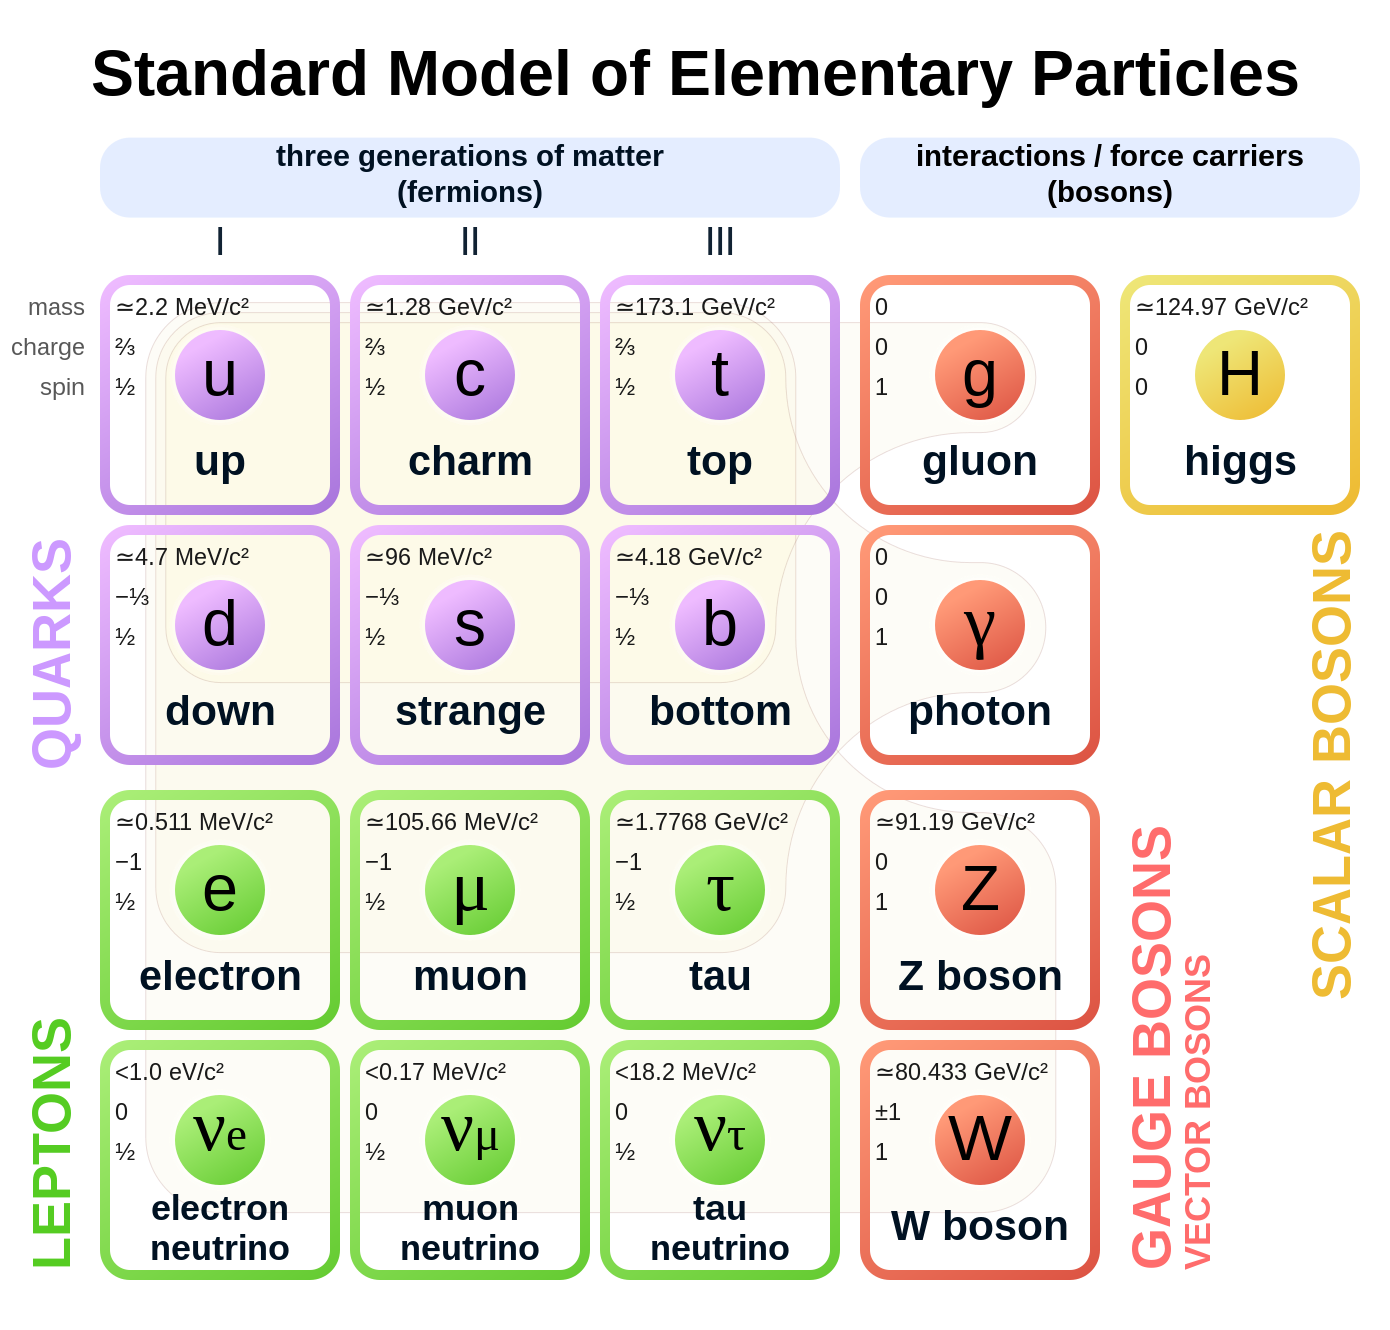
\includegraphics[width=0.6\linewidth]{figures/theory/sm.png}
	\caption{Standard model of elementary particles. Note the three generation of quarks and leptons, and their isospin doublet scheme. The four force carriers and the Higgs boson are listed on right. \cite{enwiki:1101993746}}
	\label{fig:sm}
\end{figure}

\Subsection{The Higgs Mechanism and the Higgs Boson}
The Higgs term in the Lagragian from eq. \ref{eq:lagrangian} gives rise to the mass of the gauge bosons. The potential $V(\phi)$ is given by

\begin{equation*}
	V(\phi) = -\mu^2 \phi^\dagger \phi + \frac{\lambda}{4}\left(\phi^\dagger\phi\right)^2 
\end{equation*}

and is rotational symmetric and takes a "mexican hat"-like shape. The form of the potential in the complex plane is shown if fig. \ref{fig:mexicanhat}.

\begin{figure}[h!]
	\centering
	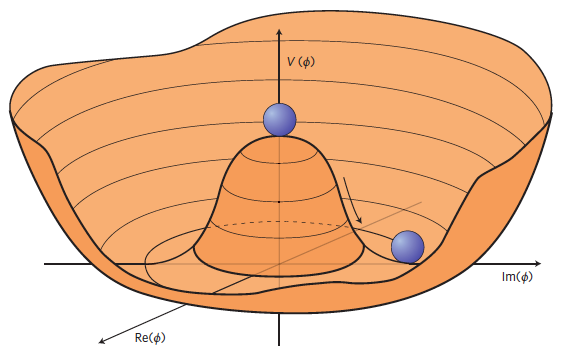
\includegraphics[width=0.8\linewidth]{figures/theory/higgspotential}
	\caption{Shape of the Higgs potential ("mexican hat"). \cite{Ellis:2012465}}
	\label{fig:mexicanhat}
\end{figure}

Due to the location of the potential minimum lying at $\phi \neq 0$ the field $\phi$ obtains a vacuum expectation value (spontaneous symmetry breaking). In addition to that, due to the covariant derivative $D_\mu$, additional coupling terms of the gauge bosons to this field $\phi$ appear. It turns out, that by writing the field $\phi$ as

\begin{equation*}
	\phi = \frac{1}{\sqrt{2}}\left(\begin{matrix}
		0 \\
		v + H
	\end{matrix}
	\right)
\end{equation*}

where $v$ is the location of the potential minimum (a constant) and $H$ is real scalar field, the electroweak gauge bosons  obtain a mass through the constant $v$

\begin{equation*}
	m^2_W = \frac{g^2 v^2}{4}, \quad m^2_Z = \frac{(g'^2 + g^2)v^2}{4}
\end{equation*}

with the electroweak coupling constants $g$, and $g'$. Additionally, the resulting Lagrangian density respects the physical symmetries

\begin{equation*}
	SU(3)_c \times SU(2)_L \times U(1)_Y
\end{equation*}

which would have broken in the absence of the field $\phi$. As symmetries in a Lagrangian imply the existence of charges, those of the Lagrangian $\mathcal{L}$ induce the colour charges, isospin charges and electric charges; the existence of the latter two is only visible through the electroweak unification.

Since its observation in 2012 at CERN \cite{Chatrchyan_2012} the properties of the Higgs boson has been extensively studied in detail. The SM Higgs a CP-even scalar of charge 0 with a measured mass of

\begin{equation*}
	m_H = 125.25 \pm 0.17 \, \text{GeV}
\end{equation*}

The most common Higgs production mechanisms at high energy colliders are shown in fig. \ref{fig:higgsproduction} \cite{Workman:2022ynf}. These are gluon-gluon fusion (ggF), vector-boson fusion (VBF), Higgs-strahlung (VH), associated gauge boson production at one loop from a gluon-gluon interaction, associated top quark pair production ($t\bar{t}H$) and associated single top quark-quark production ($tHq$).

\begin{figure}[h!]
	\centering
	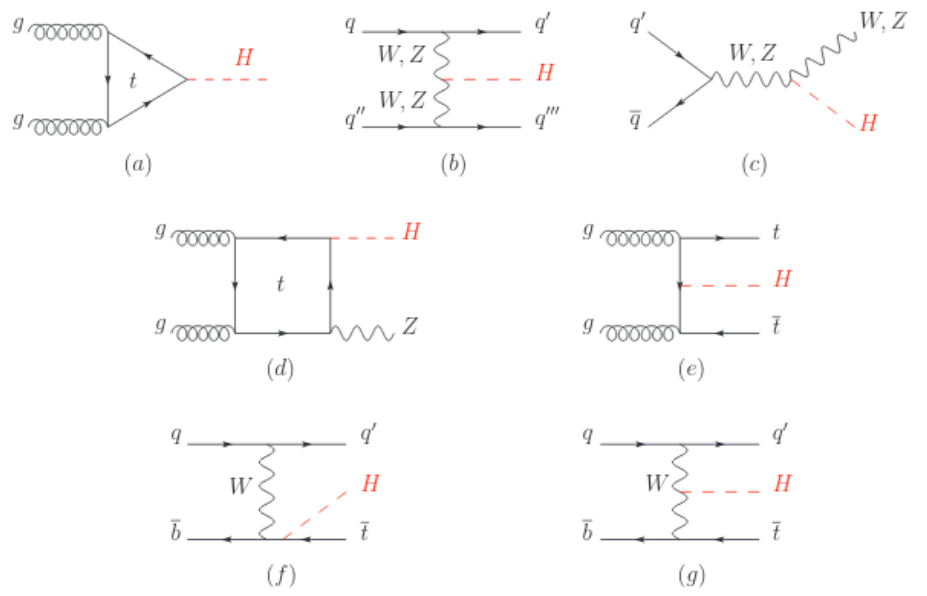
\includegraphics[width=0.8\linewidth]{figures/theory/higgsproduction.png}
	\caption{Main Higgs boson production processes in high energy hadron colliders \cite{Workman:2022ynf}.}
	\label{fig:higgsproduction}
\end{figure}

In the following the vector boson associated Higgs production will be discussed in detail.

\Subsection{VH-Higgs Production}